\section{Date: 2026-08-14}
\noindent \textbf{Series ID: EAMLXDBNQ} 

\noindent This series is titled Average Loan Size for 31 to 365 Days, Low Risk, Domestic Banks (DISCONTINUED) and has a frequency of Quarterly, 2nd Month's 1st Full Week. The units are Thousands of Dollars and the seasonal adjustment is Not Seasonally Adjusted.The observation start date is 1997-04-01 and the observation end date is 2017-04-01.The popularity of this series is 1. \\ 

\noindent \textbf{Series ID: A261RL1Q225SBEA} 

\noindent This series is titled Real Gross Domestic Income and has a frequency of Quarterly. The units are Percent Change from Preceding Period and the seasonal adjustment is Seasonally Adjusted Annual Rate.The observation start date is 1947-04-01 and the observation end date is 2026-01-01.The popularity of this series is 27. \\ 

\subsection{Raw Regression}
\noindent Regresses the two series against each other directly. A significant result here can come just as easily from both series sharing a long-run trend as from any real relationship.

\begin{center}
\begin{tabular}{lclc}
\toprule
\textbf{Dep. Variable:}         & value\_fred\_A261RL1Q225SBEA & \textbf{  R-squared:         } &     0.020   \\
\textbf{Model:}                 &             OLS              & \textbf{  Adj. R-squared:    } &     0.008   \\
\textbf{Method:}                &        Least Squares         & \textbf{  F-statistic:       } &     1.629   \\
\textbf{Date:}                  &       Fri, 14 Aug 2026       & \textbf{  Prob (F-statistic):} &    0.206    \\
\textbf{Time:}                  &           12:37:50           & \textbf{  Log-Likelihood:    } &   -202.51   \\
\textbf{No. Observations:}      &                81            & \textbf{  AIC:               } &     409.0   \\
\textbf{Df Residuals:}          &                79            & \textbf{  BIC:               } &     413.8   \\
\textbf{Df Model:}              &                 1            & \textbf{                     } &             \\
\textbf{Covariance Type:}       &          nonrobust           & \textbf{                     } &             \\
\bottomrule
\end{tabular}
\begin{tabular}{lcccccc}
                                & \textbf{coef} & \textbf{std err} & \textbf{t} & \textbf{P$> |$t$|$} & \textbf{[0.025} & \textbf{0.975]}  \\
\midrule
\textbf{const}                  &       2.9300  &        0.515     &     5.689  &         0.000        &        1.905    &        3.955     \\
\textbf{value\_fred\_EAMLXDBNQ} &      -0.0008  &        0.001     &    -1.276  &         0.206        &       -0.002    &        0.000     \\
\bottomrule
\end{tabular}
\begin{tabular}{lclc}
\textbf{Omnibus:}       & 20.575 & \textbf{  Durbin-Watson:     } &    1.219  \\
\textbf{Prob(Omnibus):} &  0.000 & \textbf{  Jarque-Bera (JB):  } &   31.073  \\
\textbf{Skew:}          & -1.046 & \textbf{  Prob(JB):          } & 1.79e-07  \\
\textbf{Kurtosis:}      &  5.198 & \textbf{  Cond. No.          } & 1.26e+03  \\
\bottomrule
\end{tabular}
%\caption{OLS Regression Results}
\end{center}

Notes: \newline
 [1] Standard Errors assume that the covariance matrix of the errors is correctly specified. \newline
 [2] The condition number is large, 1.26e+03. This might indicate that there are \newline
 strong multicollinearity or other numerical problems.

\begin{figure}
\centering
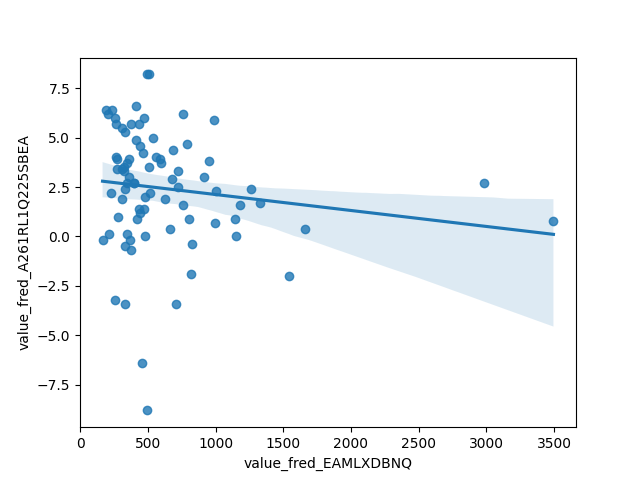
\includegraphics[scale = 0.9]{plots/plot_2026-08-14.png}
\caption{Raw Regression Plot for 2026-08-14}
\end{figure}
\newpage
\subsection{Detrended Regression}
\noindent Regresses the residuals of each series after removing its own linear time trend, so a shared trend can no longer drive the result on its own. A relationship that stays significant here is better evidence of a genuine link between the two series.

\begin{center}
\begin{tabular}{lclc}
\toprule
\textbf{Dep. Variable:}                    & value\_fred\_A261RL1Q225SBEA\_detrended & \textbf{  R-squared:         } &     0.003   \\
\textbf{Model:}                            &                   OLS                   & \textbf{  Adj. R-squared:    } &    -0.010   \\
\textbf{Method:}                           &              Least Squares              & \textbf{  F-statistic:       } &    0.2417   \\
\textbf{Date:}                             &             Fri, 14 Aug 2026            & \textbf{  Prob (F-statistic):} &    0.624    \\
\textbf{Time:}                             &                 12:37:51                & \textbf{  Log-Likelihood:    } &   -200.76   \\
\textbf{No. Observations:}                 &                      81                 & \textbf{  AIC:               } &     405.5   \\
\textbf{Df Residuals:}                     &                      79                 & \textbf{  BIC:               } &     410.3   \\
\textbf{Df Model:}                         &                       1                 & \textbf{                     } &             \\
\textbf{Covariance Type:}                  &                nonrobust                & \textbf{                     } &             \\
\bottomrule
\end{tabular}
\begin{tabular}{lcccccc}
                                           & \textbf{coef} & \textbf{std err} & \textbf{t} & \textbf{P$> |$t$|$} & \textbf{[0.025} & \textbf{0.975]}  \\
\midrule
\textbf{const}                             &    2.173e-13  &        0.325     &   6.7e-13  &         1.000        &       -0.646    &        0.646     \\
\textbf{value\_fred\_EAMLXDBNQ\_detrended} &      -0.0003  &        0.001     &    -0.492  &         0.624        &       -0.002    &        0.001     \\
\bottomrule
\end{tabular}
\begin{tabular}{lclc}
\textbf{Omnibus:}       & 21.332 & \textbf{  Durbin-Watson:     } &    1.245  \\
\textbf{Prob(Omnibus):} &  0.000 & \textbf{  Jarque-Bera (JB):  } &   33.382  \\
\textbf{Skew:}          & -1.063 & \textbf{  Prob(JB):          } & 5.64e-08  \\
\textbf{Kurtosis:}      &  5.318 & \textbf{  Cond. No.          } &     484.  \\
\bottomrule
\end{tabular}
%\caption{OLS Regression Results}
\end{center}

Notes: \newline
 [1] Standard Errors assume that the covariance matrix of the errors is correctly specified.

\begin{figure}
\centering
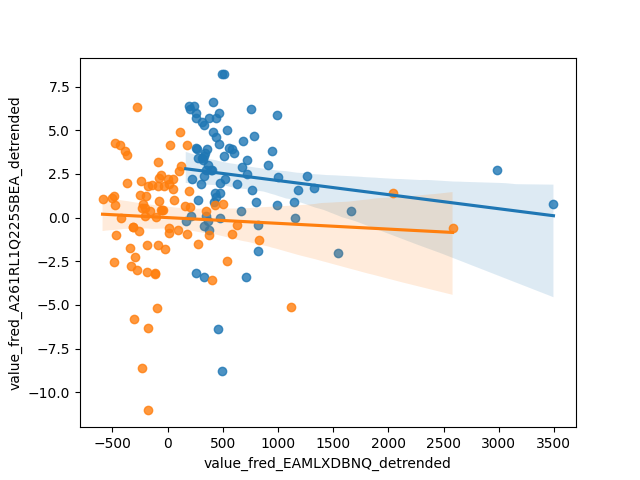
\includegraphics[scale = 0.9]{plots/plot_2026-08-14_detrended.png}
\caption{Detrended Regression Plot for 2026-08-14}
\end{figure}
\newpage
